\section{Usage}
\frame{\tableofcontents[currentsection]}

\begin{frame}
  \frametitle{Usage}
  \begin{itemize}
    \item For low level stuff
          \begin{itemize}
            \item Reading binary files
            \item Networking
            \item \dots
          \end{itemize}
    \item For optimization
          \begin{itemize}
            \item 64 bit ints can represent chess boards
            \item 9 bits can be used as sets for Sudoku solving
          \end{itemize}
  \end{itemize}
\end{frame}

\subsection{Union of Bits}
\frame{\tableofcontents[currentsubsection]}

\begin{frame}
  \frametitle{Example: Taking a union of bits}
  \begin{itemize}
    \item \texttt{a = 0x100}, \texttt{b = 0x020}, \texttt{c = 0x003}
    \item Goal: Combine \texttt{a}, \texttt{b} and \texttt{c} into one number \texttt{0x123}
  \end{itemize}
\end{frame}

\begin{frame}
  \frametitle{Example: Taking a union of bits}
  \structure{First Possibility}
  \begin{itemize}
    \item Addition
    \item \texttt{a + b + c} yields \texttt{0x123}
  \end{itemize}
  \vskip4mm
  \structure{Second Possibility}
  \begin{itemize}
    \item Bitwise or
    \item \texttt{a | b | c} also yields \texttt{0x123}
  \end{itemize}
  \vskip4mm
  \structure{Important}
  \begin{itemize}
    \item Note that \texttt{+} and \texttt{|} are not interchangeable in general!
          \begin{itemize}
            \item \texttt{1 | 1 == 1}
            \item \texttt{1 + 1 == 2}
          \end{itemize}
  \end{itemize}
\end{frame}

\begin{frame}
  \frametitle{Example: Taking a union of bits}
  \structure{Important To Understand}
  \begin{itemize}
    \item \texttt{|} is often used to combine parts into one larger whole
    \item For this, it is important that the parts don't overlap
          \begin{itemize}
            \item E.g.~\texttt{0x120 | 0x034} both use the second digit: overlap
          \end{itemize}
    \item This usage will return often
  \end{itemize}
\end{frame}

\subsection{Merging 2 Bytes}
\frame{\tableofcontents[currentsubsection]}

\begin{frame}
  \frametitle{Example: Putting 2 \texttt{uint8\_t}s In One \texttt{uint16\_t}}
  \structure{Goal}
  \begin{center}
    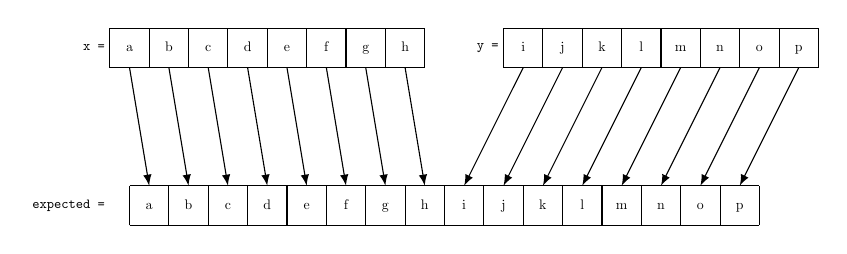
\begin{tikzpicture}
      \begin{scope}[scale=0.5,transform shape]
        \draw (0,0) grid (8,1);
        \node[anchor=east,font=\ttfamily] at (0,0.5) {x = };
        \foreach[count=\i,evaluate={\i-0.5} as \x] \v in {a,b,c,d,e,f,g,h} {
          \node[anchor=base] at (\x, 0.4) {\v};
        }
      \end{scope}
      \begin{scope}[xshift=5cm,scale=0.5,transform shape]
        \draw (0,0) grid (8,1);
        \node[anchor=east,font=\ttfamily] at (0,0.5) {y = };
        \foreach[count=\i,evaluate={\i-0.5} as \x] \v in {i,j,k,l,m,n,o,p} {
          \node[anchor=base] at (\x, 0.4) {\v};
        }
      \end{scope}

      \foreach[count=\i,evaluate={\i/2-0.25} as \x] \v in {1,...,8} {
        \draw[-latex] (\x,0) -- ++(0.25,-1.5);
        \draw[-latex] (\x+5,0) -- ++(-0.75,-1.5);
      }

      \begin{scope}[yshift=-2cm,scale=0.5,transform shape]
        \node[anchor=east,font=\ttfamily] at (0,0.5) {expected = };
        \begin{scope}[xshift=0.5cm]
          \draw (0,0) grid (16,1);
          \foreach[count=\i,evaluate={\i-0.5} as \x] \v in {a,b,c,d,e,f,g,h,i,j,k,l,m,n,o,p} {
            \node[anchor=base] at (\x, 0.4) {\v};
          }
        \end{scope}
      \end{scope}
    \end{tikzpicture}
  \end{center}
\end{frame}

\begin{frame}
  \frametitle{Example: Putting 2 \texttt{uint8\_t}s In One \texttt{uint16\_t}}
  \structure{Step 1: upgrade \texttt{a} to a \texttt{uint16\_t}}
  \begin{center}
    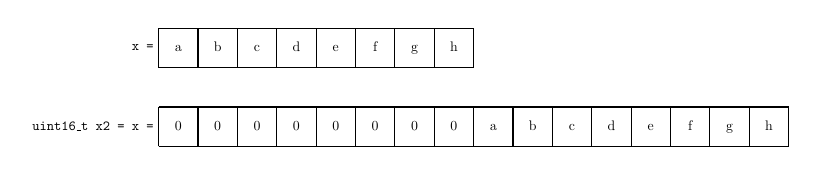
\begin{tikzpicture}
      \begin{scope}[scale=0.5,transform shape]
        \draw (0,0) grid (8,1);
        \node[anchor=east,font=\ttfamily] at (0,0.5) {x = };
        \foreach[count=\i,evaluate={\i-0.5} as \x] \v in {a,b,c,d,e,f,g,h} {
          \node[anchor=base] at (\x, 0.4) {\v};
        }
      \end{scope}
      \begin{scope}[yshift=-1cm,scale=0.5,transform shape]
        \draw (0,0) grid (16,1);
        \node[anchor=east,font=\ttfamily] at (0,0.5) {uint16\_t x2 = x = };
        \foreach[count=\i,evaluate={\i-0.5} as \x] \v in {0,0,0,0,0,0,0,0,a,b,c,d,e,f,g,h} {
          \node[anchor=base] at (\x, 0.4) {\v};
        }
      \end{scope}
    \end{tikzpicture}
  \end{center}
\end{frame}

\begin{frame}
  \frametitle{Example: Putting 2 \texttt{uint8\_t}s In One \texttt{uint16\_t}}
  \structure{Step 2: shift bits to the left}
  \begin{center}
    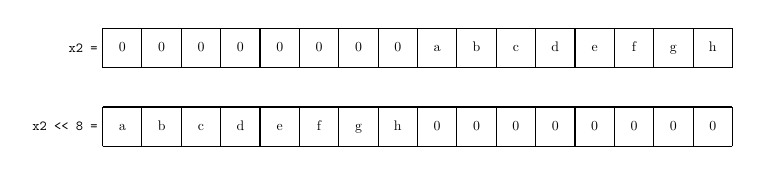
\begin{tikzpicture}
      \begin{scope}[scale=0.5,transform shape]
        \draw (0,0) grid (16,1);
        \node[anchor=east,font=\ttfamily] at (0,0.5) {x2 = };
        \foreach[count=\i,evaluate={\i-0.5} as \x] \v in {0,0,0,0,0,0,0,0,a,b,c,d,e,f,g,h} {
          \node[anchor=base] at (\x, 0.4) {\v};
        }
      \end{scope}
      \begin{scope}[yshift=-1cm,scale=0.5,transform shape]
        \draw (0,0) grid (16,1);
        \node[anchor=east,font=\ttfamily] at (0,0.5) {x2 << 8 = };
        \foreach[count=\i,evaluate={\i-0.5} as \x] \v in {a,b,c,d,e,f,g,h,0,0,0,0,0,0,0,0} {
          \node[anchor=base] at (\x, 0.4) {\v};
        }
      \end{scope}
    \end{tikzpicture}
  \end{center}
\end{frame}

\begin{frame}
  \frametitle{Example: Putting 2 \texttt{uint8\_t}s In One \texttt{uint16\_t}}
  \structure{Step 3: combine this with \texttt{b}}
  \begin{center}
    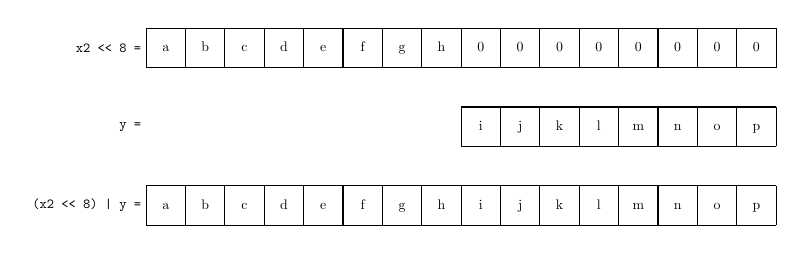
\begin{tikzpicture}
      \begin{scope}[scale=0.5,transform shape]
        \draw (0,0) grid (16,1);
        \node[anchor=east,font=\ttfamily] at (0,0.5) {x2 << 8 = };
        \foreach[count=\i,evaluate={\i-0.5} as \x] \v in {a,b,c,d,e,f,g,h,0,0,0,0,0,0,0,0} {
          \node[anchor=base] at (\x, 0.4) {\v};
        }
      \end{scope}
      \begin{scope}[yshift=-1cm,scale=0.5,transform shape]
        \node[anchor=east,font=\ttfamily] at (0,0.5) {y = };
        \begin{scope}[xshift=8cm]
          \draw (0,0) grid (8,1);
          \foreach[count=\i,evaluate={\i-0.5} as \x] \v in {i,j,k,l,m,n,o,p} {
            \node[anchor=base] at (\x, 0.4) {\v};
          }
        \end{scope}
      \end{scope}
      \begin{scope}[yshift=-2cm,scale=0.5,transform shape]
        \draw (0,0) grid (16,1);
        \node[anchor=east,font=\ttfamily] at (0,0.5) {(x2 << 8) | y = };
        \foreach[count=\i,evaluate={\i-0.5} as \x] \v in {a,b,c,d,e,f,g,h,i,j,k,l,m,n,o,p} {
          \node[anchor=base] at (\x, 0.4) {\v};
        }
      \end{scope}
    \end{tikzpicture}
  \end{center}
\end{frame}

\begin{frame}
  \frametitle{Example: Putting 2 \texttt{uint8\_t}s In One \texttt{uint16\_t}}
  \begin{itemize}
    \item Step 1 is actually redundant
    \item When shifting, values are automatically upgraded
  \end{itemize}
  \begin{center} \ttfamily
    (x << 8) | y
  \end{center}
\end{frame}

\subsection{Merging 4 Bytes}
\frame{\tableofcontents[currentsubsection]}

\begin{frame}
  \frametitle{Example: Putting 4 \texttt{uint8\_t}s In One \texttt{uint32\_t}}
  \begin{itemize}
    \item Combine four \texttt{uint8\_t a, b, c, d} into one \texttt{uint32\_t}
    \item Shift \texttt{a} 24 bits to the left
    \item Shift \texttt{b} 16 bits to the left
    \item Shift \texttt{c} 8 bits to the left
    \item Combine everything using \texttt{|}
  \end{itemize}
  \begin{center} \ttfamily
    (a << 24) | (b << 16) | (c << 8) | d
  \end{center}
\end{frame}

\subsection{Masking}
\frame{\tableofcontents[currentsubsection]}

\begin{frame}
  \frametitle{Example: Masking}
  \begin{itemize}
    \item Say we have \texttt{uint32\_t a = 0x12345678}
    \item Goal: we wish to drop cut off the first 3 bytes
    \item In other words: we want \texttt{0x00000078}
  \end{itemize}
\end{frame}

\begin{frame}
  \frametitle{Example: Masking}
  \structure{Approach}
  \begin{itemize}
    \item The bitwise and allows us to filter out bits
    \item Put differently, the \texttt{\&} can be used to "turn off" bits
  \end{itemize}
  \begin{center}
    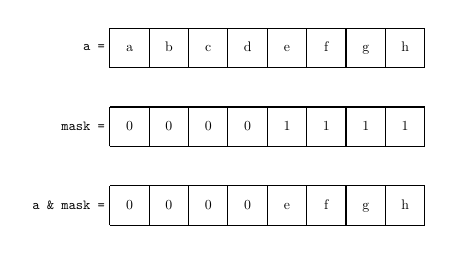
\begin{tikzpicture}
      \begin{scope}[scale=0.5,transform shape]
        \draw (0,0) grid (8,1);
        \node[anchor=east,font=\ttfamily] at (0,0.5) {a = };
        \foreach[count=\i,evaluate={\i-0.5} as \x] \v in {a,b,c,d,e,f,g,h} {
          \node[anchor=base] at (\x, 0.4) {\v};
        }
      \end{scope}
      \begin{scope}[yshift=-1cm,scale=0.5,transform shape]
        \node[anchor=east,font=\ttfamily] at (0,0.5) {mask = };
        \draw (0,0) grid (8,1);
        \foreach[count=\i,evaluate={\i-0.5} as \x] \v in {0,0,0,0,1,1,1,1} {
          \node[anchor=base] at (\x, 0.4) {\v};
        }
      \end{scope}
      \begin{scope}[yshift=-2cm,scale=0.5,transform shape]
        \draw (0,0) grid (8,1);
        \node[anchor=east,font=\ttfamily] at (0,0.5) {a \& mask = };
        \foreach[count=\i,evaluate={\i-0.5} as \x] \v in {0,0,0,0,e,f,g,h} {
          \node[anchor=base] at (\x, 0.4) {\v};
        }
      \end{scope}
    \end{tikzpicture}
  \end{center}
  \begin{itemize}
    \item The \texttt{0}s in the mask specify which bits to turn off
    \item The \texttt{1}s in the mask specify which bits to keep intact
  \end{itemize}
\end{frame}

\subsection{Extracting a Bytes}
\frame{\tableofcontents[currentsubsection]}

\begin{frame}
  \frametitle{Example: Extracting a byte from a \texttt{uint32\_t}}
  \begin{itemize}
    \item Say we have \texttt{uint32\_t a = 0x12345678}
    \item Goal: Extract the second byte from the right (\texttt{0x56})
  \end{itemize}
\end{frame}

\begin{frame}
  \frametitle{Example: Extracting a byte from a \texttt{uint32\_t}}
  \structure{Approach}
  \begin{itemize}
    \item We use a mask to keep only the relevant bits
          \begin{center} \ttfamily
            a \& 0x0000FF00
          \end{center}
    \item Reminder: \texttt{0xFF} has all bits turned on
          \begin{itemize}
            \item \texttt{0xFF == 0b11111111}
          \end{itemize}
    \item Next, we shift the relevant bits in position
          \begin{center} \ttfamily
            (a \& 0x0000FF00) >> 8
          \end{center}
  \end{itemize}
\end{frame}
